\documentclass[../general/general]{subfiles}

\begin{document}

\chapter{Лекция №6}
\noindent\textit{А.\,М.~Белемук \hfill 20 марта 2021}
\vspace{1em}


% ===== СЕКЦИЯ 1: Разложение Зоммерфельда =====
\section{Приближённое вычисление интегралов с функцией Ферми-Дирака}

Итак, у нас лекция шестая, статистическая физика. Мы продолжаем изучение идеального ферми-газа. В прошлый раз мы нашли среднее число частиц и среднюю энергию в виде интегралов, содержащих функцию Ферми-Дирака. Сегодня начнём с первого пункта: приближённое вычисление таких интегралов. Нас интересует случай низких температур $T \ll \mu$ — именно тогда мы можем найти поправки к нулевотемпературному результату.

\subsection{Постановка задачи}

Рассмотрим общий интеграл следующего вида (параметр $y = \mu/T$ считаем безразмерным):
\begin{equation}
    I(y) = \int_0^\infty \frac{f(x)}{e^{x - y} + 1}\, dx
\end{equation}
Здесь $x = \epsilon/T$ --- безразмерная энергия, $y = \mu/T$. Нас интересует случай $y \gg 1$, то есть низкие температуры при фиксированном химическом потенциале. В этом случае функция Ферми-Дирака отличается от ступеньки Хевисайда лишь в узкой полоске шириной порядка единицы вблизи $x = y$, и мы можем систематически учесть это отличие.

\subsection{Вывод разложения Зоммерфельда}

Разобьём интеграл $I(y)$ на три части, добавив и вычтя нужные слагаемые:
\begin{equation}
    I(y) = \int_0^y f(x)\, dx + \int_0^y f(x)\!\left[\frac{1}{e^{x-y}+1} - 1\right] dx + \int_y^\infty \frac{f(x)}{e^{x-y}+1}\, dx
\end{equation}

Первый интеграл --- это «нулевотемпературный» результат (как если бы $n_F$ была ступенькой). Заметим, что $\frac{1}{e^{x-y}+1} - 1 = -\frac{1}{e^{y-x}+1}$. Тогда два последних интеграла образуют поправку $\delta I$:
\begin{equation}
    \delta I = -\int_0^y \frac{f(x)}{e^{y-x}+1}\, dx + \int_y^\infty \frac{f(x)}{e^{x-y}+1}\, dx
\end{equation}

В первом интеграле делаем замену $z = y - x$ (то есть $x = y - z$, $dx = -dz$). Поскольку $y \gg 1$, а подынтегральная функция при $z \gg 1$ экспоненциально мала, верхний предел можно с экспоненциальной точностью заменить на $+\infty$:
\begin{equation}
    -\int_0^y \frac{f(y-z)}{e^z+1}\, dz \approx -\int_0^\infty \frac{f(y-z)}{e^z+1}\, dz
\end{equation}

Во втором интеграле делаем замену $z = x - y$ ($x = y + z$, $dx = dz$):
\begin{equation}
    \int_0^\infty \frac{f(y+z)}{e^z+1}\, dz
\end{equation}

Складывая, получаем:
\begin{equation}
    \delta I \approx \int_0^\infty \frac{f(y+z) - f(y-z)}{e^z+1}\, dz
\end{equation}

Существенный вклад в интеграл дают только $z \lesssim 1$, поэтому раскладываем по Тейлору вокруг точки $y$:
\begin{equation}
    f(y+z) - f(y-z) = 2z\,f'(y) + \frac{2z^3}{3!}\,f'''(y) + \ldots
\end{equation}
Чётные члены разложения сокращаются, остаются только нечётные. Подставляем и берём первый нетривиальный член:
\begin{equation}
    \delta I \approx 2f'(y) \int_0^\infty \frac{z}{e^z+1}\, dz + \ldots
\end{equation}

Стоящий здесь интеграл является точно вычислимой константой:
\begin{equation}
    \int_0^\infty \frac{z}{e^z+1}\, dz = \frac{\pi^2}{12}
\end{equation}

Следовательно, $\delta I \approx \frac{\pi^2}{6}\,f'(y)$. Собирая всё вместе, получаем результат, который называется \textbf{разложением Зоммерфельда}:
\begin{equation}
    \boxed{I(y) = \int_0^y f(x)\, dx + \frac{\pi^2}{6}\, f'(y) + O(y^{-4})}
\end{equation}

\subsection{Форма разложения в исходных переменных}

Возвращаясь к исходным переменным ($x = \epsilon/T$, $y = \mu/T$), разложение Зоммерфельда принимает вид:
\begin{equation}
    \int_0^\infty \frac{f(\epsilon)}{e^{(\epsilon-\mu)/T}+1}\, d\epsilon = \int_0^\mu f(\epsilon)\, d\epsilon + \frac{\pi^2 T^2}{6}\, f'(\mu) + O\!\left(\frac{T^4}{\mu^4}\right)
    \label{eq:sommerfeld}
\end{equation}
Это наш основной инструмент на сегодня. Прошу запомнить: разложение Зоммерфельда очень часто используется в физике конденсированного состояния при низких температурах.

% ===== КОНЕЦ СЕКЦИИ 1 =====


% ===== СЕКЦИЯ 2: Химический потенциал ферми-газа при конечных температурах =====
\section{Химический потенциал ферми-газа при низких температурах}

\subsection{Уравнение для числа частиц}

Вернёмся к уравнению на число частиц. В прошлый раз при $T = 0$ мы вычислили его и получили:
\begin{equation}
    N = \frac{2A}{3}\, \epsilon_F^{3/2}
\end{equation}
Теперь рассматриваем случай конечных, но малых температур: $T \ll \epsilon_F$. Уравнение на $N$ принимает вид:
\begin{equation}
    N = \int_0^\infty \nu(\epsilon)\, n_F(\epsilon)\, d\epsilon = \int_0^\infty \frac{A\sqrt{\epsilon}}{e^{(\epsilon-\mu)/T}+1}\, d\epsilon
\end{equation}

\subsection{Применение разложения Зоммерфельда}

Применяем формулу~\eqref{eq:sommerfeld}, полагая $f(\epsilon) = \nu(\epsilon) = A\sqrt{\epsilon}$. Тогда $f'(\epsilon) = \frac{A}{2\sqrt{\epsilon}}$. Подставляя:
\begin{equation}
    N = \int_0^\mu A\sqrt{\epsilon}\, d\epsilon + \frac{\pi^2 T^2}{6} \cdot \frac{A}{2\sqrt{\mu}} + \ldots = \frac{2A}{3}\, \mu^{3/2} + \frac{\pi^2 A T^2}{12\sqrt{\mu}} + \ldots
\end{equation}

Вынесем за скобку $\frac{2A}{3}\mu^{3/2}$:
\begin{equation}
    N = \frac{2A}{3}\, \mu^{3/2} \left( 1 + \frac{\pi^2 T^2}{8\mu^2} + \ldots \right)
\end{equation}

Поскольку слева стоит $N = \frac{2A}{3}\epsilon_F^{3/2}$, получаем:
\begin{equation}
    \left(\frac{\epsilon_F}{\mu}\right)^{3/2} = 1 + \frac{\pi^2 T^2}{8\mu^2} + \ldots
    \quad \text{или} \quad
    1 = \left(\frac{\mu}{\epsilon_F}\right)^{3/2}\!\!\left(1 + \frac{\pi^2 T^2}{8\mu^2} + \ldots\right)
\end{equation}

\subsection{Нахождение $\mu(T)$}

Ищем температурную поправку к $\mu$:
\begin{equation}
    \mu = \epsilon_F\!\left(1 + c\frac{T^2}{\epsilon_F^2} + \ldots\right)
\end{equation}
Так как поправка мала, в знаменателе $8\mu^2$ можно сразу заменить $\mu \to \epsilon_F$. Подставляем и раскладываем до порядка $(T/\epsilon_F)^2$:
\begin{equation}
    1 = \left(1 + \frac{3c}{2}\frac{T^2}{\epsilon_F^2}\right)\!\left(1 + \frac{\pi^2 T^2}{8\epsilon_F^2}\right) \approx 1 + \frac{3c}{2}\frac{T^2}{\epsilon_F^2} + \frac{\pi^2 T^2}{8\epsilon_F^2}
\end{equation}
Чтобы это тождество выполнялось, коэффициент при $T^2/\epsilon_F^2$ должен быть равен нулю:
\begin{equation}
    \frac{3c}{2} + \frac{\pi^2}{8} = 0 \quad \Longrightarrow \quad c = -\frac{\pi^2}{12}
\end{equation}

Итоговый важнейший результат --- зависимость химического потенциала ферми-газа от температуры (формула~2):
\begin{equation}
    \boxed{\mu(T) = \epsilon_F\left[1 - \frac{\pi^2}{12}\left(\frac{T}{\epsilon_F}\right)^2 + O\!\left(\frac{T^4}{\epsilon_F^4}\right)\right]}
    \label{eq:mu_fermi}
\end{equation}

\subsection{График зависимости $\mu(T)$}

\begin{figure}[h!]
    \centering
    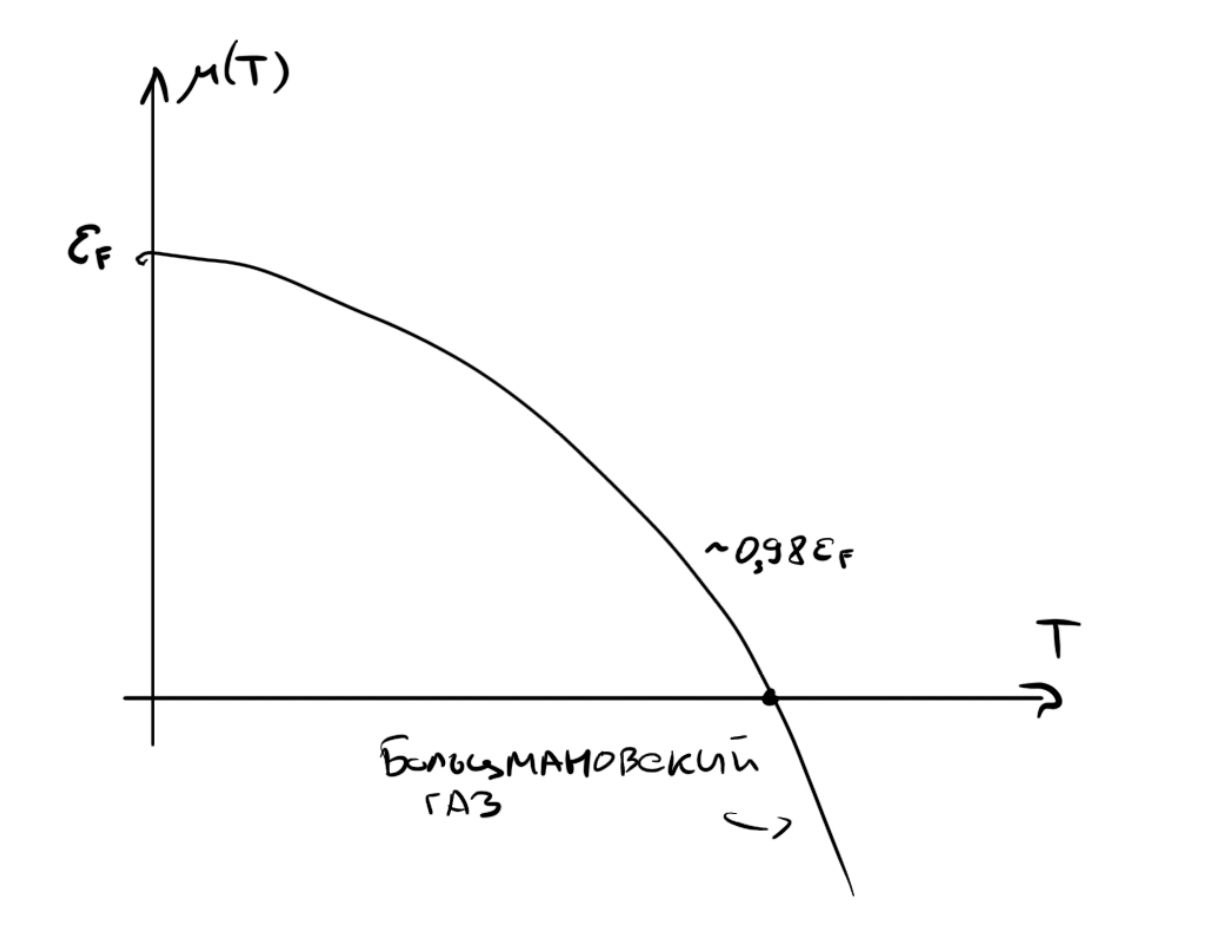
\includegraphics[width=\textwidth]{images/mu.jpg}
    \caption{Химический потенциал ферми-газа как функция температуры при фиксированной плотности.}
\end{figure}

При $T = 0$ химический потенциал равен энергии Ферми. При малых $T$ он убывает пропорционально $T^2$. При $T \approx 0{,}98\,\epsilon_F$ обращается в нуль, а при высоких температурах уходит в классический предел $\mu = T\ln(nV_Q) \to -\infty$.

% ===== КОНЕЦ СЕКЦИИ 2 =====


% ===== СЕКЦИЯ 3: Энергия и теплоёмкость ферми-газа =====
\section{Энергия и теплоёмкость идеального ферми-газа}

\subsection{Энергия при $T = 0$}

Следующий пункт --- зависимость энергии от температуры. Начнём с $T = 0$. Подставляя $n_F = \theta(\epsilon_F - \epsilon)$:
\begin{equation}
    E_0 = \int_0^{\epsilon_F} \epsilon\,\nu(\epsilon)\, d\epsilon = A\int_0^{\epsilon_F} \epsilon^{3/2}\, d\epsilon = \frac{2A}{5}\,\epsilon_F^{5/2}
\end{equation}
Это можно переписать через $N = \frac{2A}{3}\epsilon_F^{3/2}$ и через плотность состояний на поверхности Ферми $\nu(\epsilon_F) = A\sqrt{\epsilon_F}$:
\begin{equation}
    E_0 = \frac{2A}{5}\,\epsilon_F^{5/2} = \frac{3}{5}\, N\epsilon_F = \frac{2}{5}\,\epsilon_F\,\nu(\epsilon_F)\cdot\epsilon_F
    \label{eq:E0}
\end{equation}
Запомним: $E_0 = \frac{3}{5}N\epsilon_F$ --- энергия основного состояния (энергия заполненной сферы Ферми).

\subsection{Высокотемпературный предел}

Мимоходом отметим: при $T \gg \epsilon_F$ ферми-газ переходит в классический, и его средняя энергия стремится к:
\begin{equation}
    E \xrightarrow{T \gg \epsilon_F} \frac{3}{2}\, NT
\end{equation}
что соответствует теореме о равнораспределении.

\subsection{Низкотемпературный случай: применение разложения Зоммерфельда}

Рассмотрим наиболее интересный случай $T \ll \epsilon_F$. Применяем формулу~\eqref{eq:sommerfeld} к интегралу для энергии, полагая $f(\epsilon) = \epsilon\cdot\nu(\epsilon) = A\epsilon^{3/2}$, тогда $f'(\epsilon) = \frac{3A}{2}\sqrt{\epsilon}$:
\begin{equation}
    E = \int_0^\mu A\epsilon^{3/2}\, d\epsilon + \frac{\pi^2 T^2}{6}\cdot\frac{3A}{2}\sqrt{\mu} + \ldots = \frac{2A}{5}\,\mu^{5/2} + \frac{\pi^2 A T^2}{4}\sqrt{\mu} + \ldots
\end{equation}
Вынесем за скобку $\frac{2A}{5}\mu^{5/2}$:
\begin{equation}
    E = \frac{2A}{5}\,\mu^{5/2}\!\left(1 + \frac{5\pi^2 T^2}{8\mu^2} + \ldots\right)
\end{equation}

Теперь подставляем $\mu(T)$ из формулы~\eqref{eq:mu_fermi}. Вычисляем нужную степень:
\begin{equation}
    \left(\frac{\mu}{\epsilon_F}\right)^{5/2} = \left(1 - \frac{\pi^2 T^2}{12\epsilon_F^2}\right)^{5/2} \approx 1 - \frac{5\pi^2 T^2}{24\epsilon_F^2}
\end{equation}
В малой поправке $\frac{5\pi^2 T^2}{8\mu^2}$ можно сразу заменить $\mu \approx \epsilon_F$. Перемножаем скобки:
\begin{equation}
    E = E_0\!\left(1 - \frac{5\pi^2 T^2}{24\epsilon_F^2} + \frac{5\pi^2 T^2}{8\epsilon_F^2}\right) = E_0\!\left(1 + \frac{5\pi^2 T^2}{12\epsilon_F^2}\right)
\end{equation}
(поскольку $-\frac{5}{24} + \frac{5}{8} = \frac{5}{12}$). Итоговая формула (формула~3):
\begin{equation}
    \boxed{E(T) = E_0\!\left(1 + \frac{5\pi^2}{12}\left(\frac{T}{\epsilon_F}\right)^2 + O\!\left(\frac{T^4}{\epsilon_F^4}\right)\right)}
    \label{eq:energy_fermi}
\end{equation}

\subsection{Теплоёмкость ферми-газа}

Дифференцируем формулу~\eqref{eq:energy_fermi} по температуре:
\begin{equation}
    C_V = \frac{dE}{dT} = E_0 \cdot \frac{5\pi^2}{6}\frac{T}{\epsilon_F^2} = \frac{\pi^2}{2}\,\frac{NT}{\epsilon_F}
\end{equation}

Через плотность состояний на поверхности Ферми $\nu(\epsilon_F) = \frac{3N}{2\epsilon_F}$:
\begin{equation}
    C_V = \frac{\pi^2}{3}\,\nu(\epsilon_F)\,T
\end{equation}

Главный вывод: \textbf{теплоёмкость вырожденного ферми-газа пропорциональна температуре}, $C_V = \gamma T$, где:
\begin{equation}
    \gamma = \frac{\pi^2}{3}\,\nu(\epsilon_F)
\end{equation}

\begin{figure}[h!]
    \centering
    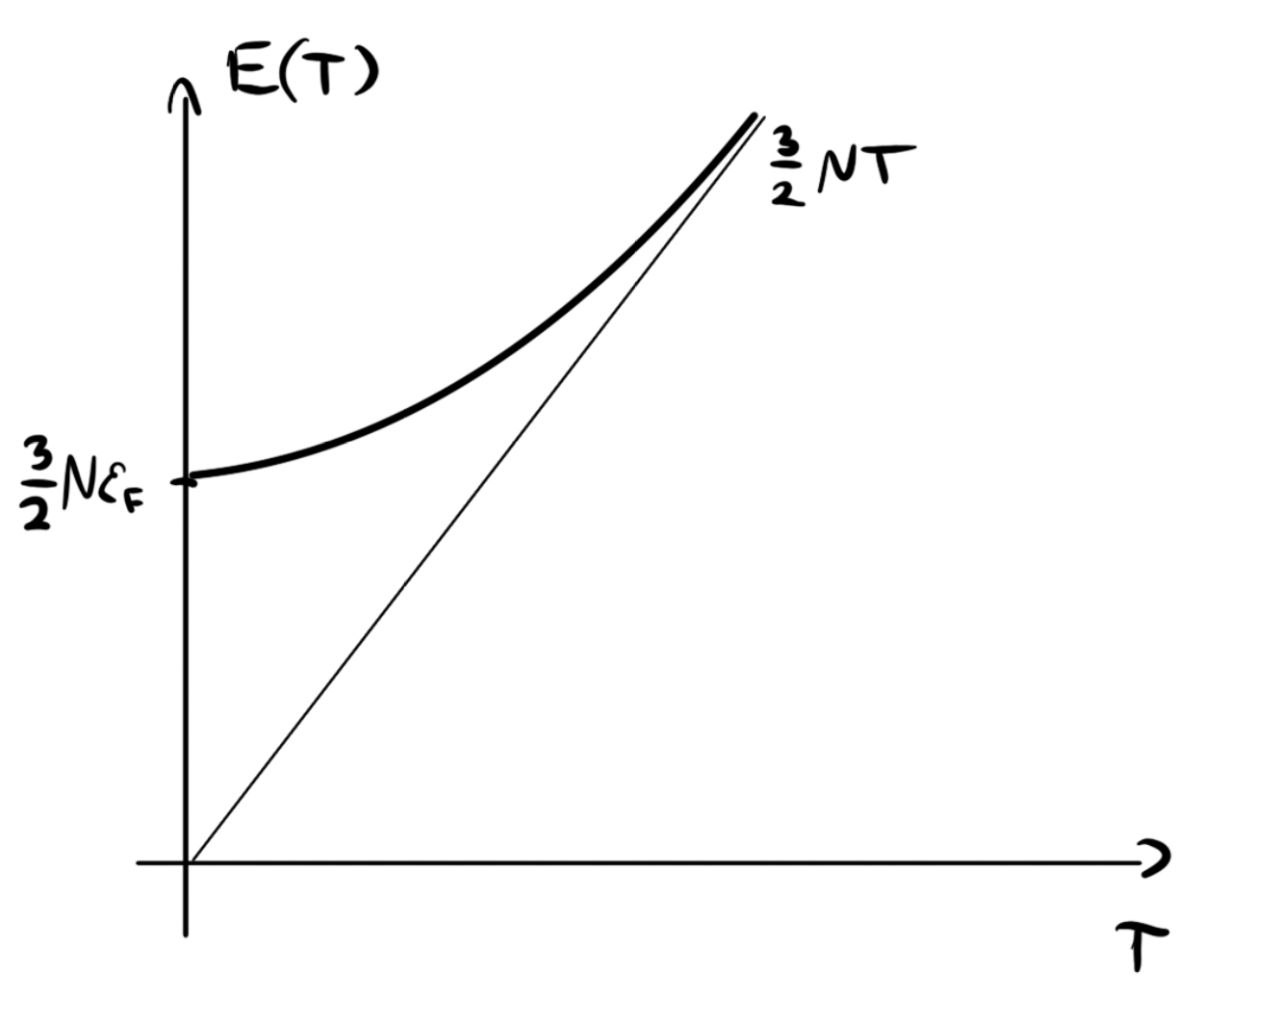
\includegraphics[width=0.7\textwidth]{images/E.jpg}
    \caption{Средняя энергия ферми-газа в зависимости от температуры. Опечатка: $3/5 N \varepsilon_F$}
\end{figure}

\subsection{Физическая интерпретация линейной теплоёмкости}

Почему $C_V \propto T$? Качественная аргументация: при нагревании размывается функция распределения Ферми-Дирака в узкой полоске шириной $\sim T$ около поверхности Ферми. Число «термически активных» электронов, способных перейти на более высокие уровни, порядка $\nu(\epsilon_F)\cdot T$. Каждый такой электрон при нагревании на $dT$ получает энергию $\sim dT$. Следовательно:
\begin{equation}
    C_V = \frac{dE}{dT} \sim \nu(\epsilon_F)\cdot T
\end{equation}

Все «глубокие» электроны, далёкие от поверхности Ферми, не могут участвовать в теплообмене --- все ближние уровни уже заняты, переходить некуда. Именно поэтому теплоёмкость металлов при низких температурах линейна по $T$ и намного меньше классического значения $\frac{3}{2}N$.

% ===== КОНЕЦ СЕКЦИИ 3 =====


% ===== СЕКЦИЯ 4: Уравнение состояния идеального ферми-газа =====
\section{Уравнение состояния идеального ферми-газа}

Мы вычислили $\mu(T)$ и $E(T)$. Теперь поставим точку --- найдём уравнение состояния, то есть давление как функцию температуры и плотности.

\subsection{Связь $\Omega$-потенциала с энергией}

Запишем $\Omega$-потенциал через большую статистическую сумму:
\begin{equation}
    \Omega = -T\ln\mathcal{Z} = -T\sum_{\vec{p},\sigma} \ln\!\left(1 + e^{(\mu - \epsilon_p)/T}\right)
\end{equation}

Переходим к интегрированию (уровни от $\sigma$ не зависят):
\begin{equation}
    \Omega = -T\int_0^\infty \nu(\epsilon)\,\ln\!\left(1 + e^{(\mu-\epsilon)/T}\right) d\epsilon = -T\!\int_0^\infty A\sqrt{\epsilon}\,\ln\!\left(1 + e^{(\mu-\epsilon)/T}\right) d\epsilon
\end{equation}

Интегрируем по частям. Обозначим:
\begin{equation}
    u = \ln\!\left(1 + e^{(\mu-\epsilon)/T}\right),
    \quad dv = A\sqrt{\epsilon}\, d\epsilon, \quad v = \frac{2A}{3}\,\epsilon^{3/2}
\end{equation}

Вычислим $du/d\epsilon$:
\begin{equation}
    \frac{du}{d\epsilon} = -\frac{1}{T}\cdot\frac{e^{(\mu-\epsilon)/T}}{1+e^{(\mu-\epsilon)/T}} = -\frac{n_F(\epsilon)}{T}
\end{equation}
Граничный член $\left[\frac{2A}{3}\epsilon^{3/2}\ln(\ldots)\right]_0^\infty$ обращается в нуль на обоих пределах. Поэтому:
\begin{equation}
    \Omega = -T\!\left(-\int_0^\infty \frac{2A}{3}\,\epsilon^{3/2}\cdot\!\left(-\frac{n_F(\epsilon)}{T}\right) d\epsilon\right) = -\frac{2}{3}\int_0^\infty A\epsilon^{3/2}\,n_F(\epsilon)\, d\epsilon
\end{equation}

Стоящий интеграл --- это в точности средняя энергия $E$. Следовательно:
\begin{equation}
    \Omega = -\frac{2}{3}\,E
    \label{eq:Omega_E}
\end{equation}

\subsection{Уравнение состояния: $PV = \frac{2}{3}E$}

Из термодинамического соотношения $\Omega = -PV$ немедленно получаем:
\begin{equation}
    \boxed{PV = \frac{2}{3}\,E}
    \label{eq:PV_E}
\end{equation}

Это соотношение справедливо при \emph{любой} температуре и является \emph{универсальным} для невзаимодействующего нерелятивистского идеального газа --- как ферми-газа, так и бозе-газа. Вывод опирается лишь на квадратичный закон дисперсии $\epsilon = p^2/(2m)$.

\subsection{Уравнение состояния при высоких температурах}

При $T \gg \epsilon_F$ используем $E = \frac{3}{2}NT$:
\begin{equation}
    PV = \frac{2}{3}\cdot\frac{3}{2}\,NT = NT \quad \Longrightarrow \quad P = nT
\end{equation}
Это уравнение состояния идеального классического газа.

\subsection{Уравнение состояния при низких температурах}

При $T \ll \epsilon_F$ подставляем формулу~\eqref{eq:energy_fermi}:
\begin{equation}
    P = \frac{2E_0}{3V}\!\left(1 + \frac{5\pi^2 T^2}{12\epsilon_F^2}\right)
\end{equation}
Обозначим давление при $T = 0$ как $P_0$:
\begin{equation}
    P_0 = \frac{2E_0}{3V} = \frac{2}{3V}\cdot\frac{3}{5}\,N\epsilon_F = \frac{2}{5}\,n\epsilon_F
\end{equation}
Тогда уравнение состояния вырожденного идеального ферми-газа:
\begin{equation}
    \boxed{P = P_0\!\left(1 + \frac{5\pi^2}{12}\frac{T^2}{\epsilon_F^2} + \ldots\right)}
\end{equation}

Подчеркнём: давление $P_0 \neq 0$ даже при $T = 0$. Это \textbf{квантовое давление} --- прямое следствие принципа Паули. Фермионы вынуждены занимать высокоэнергетические состояния, что создаёт давление даже в отсутствие тепловых флуктуаций. Именно это квантовое давление удерживает белые карлики и нейтронные звёзды от гравитационного коллапса.

Из $\epsilon_F \propto n^{2/3}$ следует $P_0 = \frac{2}{5}n\epsilon_F \propto n^{5/3}$. Изотерма при низких температурах:
\begin{equation}
    P \propto \frac{1}{V^{5/3}} \quad (T \ll \epsilon_F)
\end{equation}

\begin{figure}[h!]
    \centering
    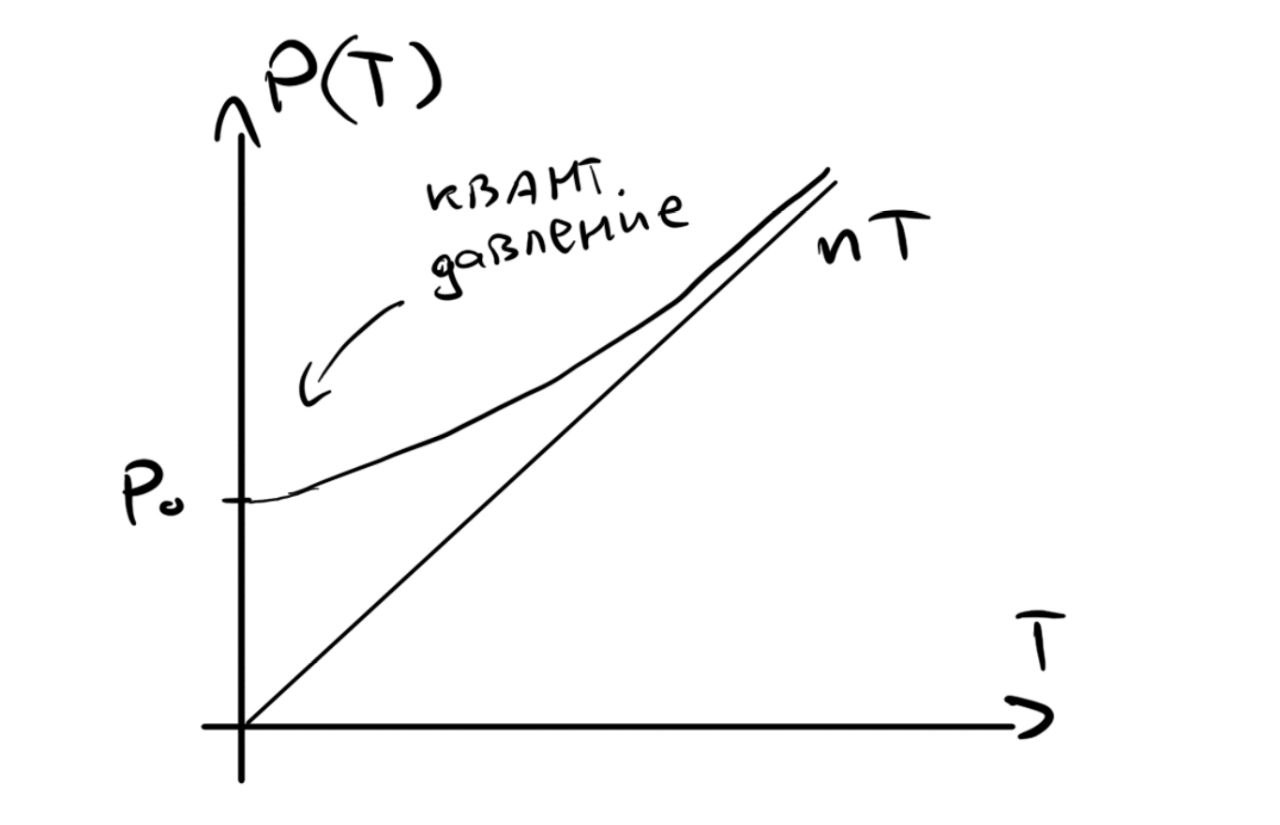
\includegraphics[width=0.7\textwidth]{images/sost.jpg}
    \caption{Уравнение состояния идеального ферми-газа.}
\end{figure}

% ===== КОНЕЦ СЕКЦИИ 4 =====


% ===== СЕКЦИЯ 5: Идеальный бозе-газ =====
\section{Большой канонический ансамбль для идеального бозе-газа}

С ферми-газом мы в основном разобрались. Теперь переходим к новой теме --- идеальный бозе-газ. Здесь есть как схожести с ферми-газом (при высоких температурах), так и принципиальные отличия: бозоны могут накапливаться в одном квантовом состоянии, что порождает явление бозе-конденсации.

\subsection{Вычисление статистической суммы: метод одного уровня}

Рассмотрим систему невзаимодействующих бозонов в ящике объёма $V$. Для простоты возьмём бозоны с нулевым спином ($g = 1$).

Применим следующий подход. Выделим из всей системы один конкретный одночастичный уровень с импульсом $\vec{p}$ и энергией $\epsilon_p$. Этот уровень будем считать «системой», а все остальные уровни --- «средой» (термостатом), задающей температуру $T$ и химический потенциал $\mu$. Применяем формализм Большого канонического ансамбля к этой маленькой «системе».

Какие квантовые состояния имеет наша «система»? Для бозонов --- любое целое число заполнения без ограничений:
\begin{itemize}
    \item $n_p = 0$: на уровне нет частиц, энергия $0$
    \item $n_p = 1$: одна частица, энергия $\epsilon_p$
    \item $n_p = 2$: две частицы, энергия $2\epsilon_p$
    \item \ldots и так далее до бесконечности
\end{itemize}

Большая статистическая сумма для этого одного уровня:
\begin{equation}
    Z_p = \sum_{n_p=0}^\infty e^{(\mu - \epsilon_p) n_p / T} = \sum_{n_p=0}^\infty \left(e^{(\mu-\epsilon_p)/T}\right)^{n_p}
\end{equation}
Это геометрическая прогрессия со знаменателем $q = e^{(\mu-\epsilon_p)/T}$. Для сходимости необходимо $|q| < 1$, то есть:
\begin{equation}
    e^{(\mu - \epsilon_p)/T} < 1 \quad \Longleftrightarrow \quad \mu < \epsilon_p \quad \forall\,\vec{p}
\end{equation}

Это условие должно выполняться для любого импульса $\vec{p}$, в том числе при $p \to 0$, когда $\epsilon_p \to 0$. Следовательно, химический потенциал бозе-газа обязан быть строго отрицательным:
\begin{equation}
    \mu < 0
\end{equation}
Это принципиальное ограничение, которого нет у ферми-газа.

Суммируем геометрическую прогрессию:
\begin{equation}
    Z_p^{BE} = \frac{1}{1 - e^{(\mu-\epsilon_p)/T}}
    \label{eq:Zp_BE}
\end{equation}

\subsection{Полная статистическая сумма}

Поскольку частицы не взаимодействуют, полная большая статистическая сумма системы равна произведению статсумм по всем одночастичным состояниям:
\begin{equation}
    \mathcal{Z}^{BE} = \prod_{\vec{p}} Z_p^{BE} = \prod_{\vec{p}} \frac{1}{1 - e^{(\mu-\epsilon_p)/T}}
\end{equation}

Этот же результат получается «в лоб» --- суммируя по всем наборам чисел заполнения $\{n_p\}$ (каждое $n_p = 0, 1, 2, \ldots$): схема вычисления один к одному такая же, как для ферми-газа, только значения $n_p$ не ограничены. Получается тот же самый результат.

\subsection{Распределение Бозе-Эйнштейна}

Среднее число частиц на состоянии $\vec{p}$ находим стандартным образом:
\begin{equation}
    \langle n_p\rangle = T\frac{\partial}{\partial\mu}\ln Z_p^{BE} = T\frac{\partial}{\partial\mu}\!\left[-\ln\!\left(1 - e^{(\mu-\epsilon_p)/T}\right)\right]
\end{equation}
Вычисляем производную и умножаем числитель и знаменатель на $e^{(\epsilon_p-\mu)/T}$:
\begin{equation}
    \langle n_p\rangle = T\cdot\frac{e^{(\mu-\epsilon_p)/T}/T}{1 - e^{(\mu-\epsilon_p)/T}} = \frac{1}{e^{(\epsilon_p - \mu)/T} - 1}
\end{equation}

Это знаменитая \textbf{функция распределения Бозе-Эйнштейна}:
\begin{equation}
    n_{BE}(\epsilon) = \frac{1}{e^{(\epsilon-\mu)/T} - 1}
\end{equation}

В знаменателе стоит «$-1$» в отличие от «$+1$» у Ферми-Дирака. При $\epsilon \to \mu$ ($\mu < 0$) функция может стать сколь угодно большой --- это отражает возможность макроскопического заполнения одного уровня.

\subsection{Уравнение на среднее число частиц и бозе-интегралы}

Суммируем по всем состояниям. Поскольку функция зависит только от $\epsilon_p = p^2/(2m)$, переходим к интегрированию по энергии:
\begin{equation}
    \langle N\rangle = \sum_{\vec{p}} n_{BE}(\epsilon_p) = \int_0^\infty \frac{\nu(\epsilon)}{e^{(\epsilon-\mu)/T}-1}\, d\epsilon = A\int_0^\infty \frac{\sqrt{\epsilon}}{e^{(\epsilon-\mu)/T}-1}\, d\epsilon
\end{equation}

Вводим безразмерные переменные $x = \epsilon/T$ и $y = -\mu/T > 0$ (заметьте: $y > 0$ согласно условию $\mu < 0$):
\begin{equation}
    \langle N\rangle = A\,T^{3/2} \int_0^\infty \frac{\sqrt{x}}{e^{x+y}-1}\, dx
\end{equation}

Для удобства введём семейство \textbf{бозе-интегралов}:
\begin{equation}
    I_\alpha(y) = \int_0^\infty \frac{x^\alpha}{e^{x+y} - 1}\, dx, \quad y > 0
\end{equation}

Тогда:
\begin{equation}
    \langle N\rangle = A\,T^{3/2}\, I_{1/2}(y)
    \label{eq:N_bose}
\end{equation}

Отличие от аналогичных ферми-интегралов --- только знак $(-1)$ вместо $(+1)$ в знаменателе. Однако именно это маленькое отличие влечёт за собой огромные последствия.

Оказывается, функция $I_{1/2}(y)$ при $y \to 0^+$ достигает конечного предела. Это означает, что при фиксированном $N$ и понижении температуры уравнение~\eqref{eq:N_bose} при некотором $T = T_c$ перестаёт иметь решение при $y > 0$. Что происходит при $T < T_c$ --- и есть \textbf{бозе-эйнштейновская конденсация}. В следующий раз мы детально исследуем поведение $I_\alpha(y)$, найдём критическую температуру и выясним физическую картину конденсации. На сегодня всё.

% ===== КОНЕЦ СЕКЦИИ 5 =====


\end{document}
